\section{Alimentação} % (fold)
\label{sub:alimentação}
	A equipe de engenharia de energia tem como dimensionar e definir o sistema de alimentação para o funcionamento do robô aspirador. Existem diversas possibilidades de fornecer a energia necessária pra suprir a potência requerida pelo sistema. A forma mais usual é a utilização de baterias.

	A fonte de alimentação ideal para o sistema segue alguns requisitos essenciais, como ter autonomia mínima de 30 minutos (tempo suficiente para aspirar um cômodo). Alguns parâmetros como tensão e corrente ainda não podem ser definidos nesta etapa do projeto. Para as alternativas disponíveis dentro desse universo têm-se como opção as baterias NIMH, que apresentam variações com diferentes valores de tensão e corrente.
	
	A recarga dessas baterias varia de acordo com o valor de potência fornecida. Alguns fabricantes produzem carregadores que retiram a tensão alternada de 220v, 60Hz para a tensão contínua da bateria escolhida. O manual do carregador informa que o tempo máximo de recarga é de 45 minutos para os modelos mais potentes de bateria, este número pode ser reduzido para 15 minutos em alguns casos. Dentre as opções disponíveis estão dispostas três nas imagens abaixo (18v, 14.4v e 12.4v/ 3,3Ah e 2,6Ah).

	\begin{figure}[H]
		\centering
		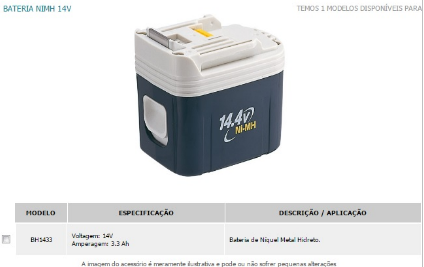
\includegraphics[scale=0.55]{figuras/bateria_1.png}
		\caption{Bateria de 14.4v.}
		\label{img:bateria_1}
	\end{figure}

	\begin{figure}[H]
		\centering
		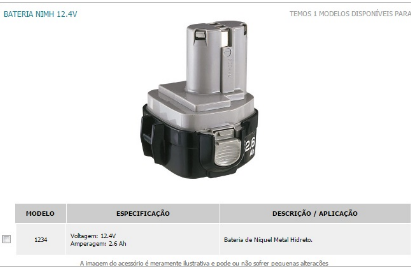
\includegraphics[scale=0.55]{figuras/bateria_2.png}
		\caption{Bateria de 12.4v.}
		\label{img:bateria_2}
	\end{figure}
	
	\begin{figure}[H]
		\centering
		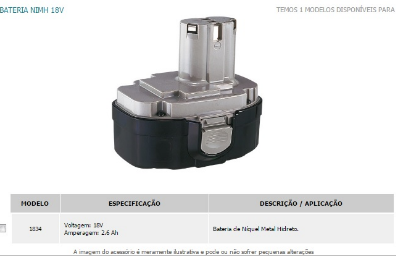
\includegraphics[scale=0.55]{figuras/bateria_3.png}
		\caption{Bateria de 18v.}
		\label{img:bateria_3}
	\end{figure}

	Outra alternativa para alimentar o aspirador é o uso de supercapacitores. Esta opção oferece valores consideravelmente maiores de ciclos de carga (10 000 contra 400-6000). Além disso, o tempo de recarga é reduzido se comparado com as baterias convencionais. A fragilidade que acarreta em um maior cuidado no manuseio, o elevado custo de mercado e a falta de informações técnicas disponíveis são algumas desvantagens ligadas ao uso de supercapacitores.
% section alimentação (end)
